\documentclass[12pt, a4paper]{article}
\usepackage[utf8]{inputenc}
%\usepackage[IL2]{fontenc}
\usepackage[czech]{babel}
\usepackage[pdftex]{graphicx}
\usepackage{mathtools}
\usepackage{amsmath}
\usepackage{svg}
\usepackage{textcomp}
\usepackage{listings,xcolor}
\usepackage[final]{pdfpages}
\usepackage{verbatim}
\usepackage{fancyhdr}
\usepackage[T1]{fontenc}

\usepackage[nottoc,notlot,notlof]{tocbibind}
\usepackage[pdftex,hypertexnames=false]{hyperref}
\hypersetup{colorlinks=true,
  unicode=true,
  linkcolor=black,
  citecolor=black,
  urlcolor=black,
  bookmarksopen=true}

\title{\textbf{Dokumentace semestrální práce} \\KIV/PT}
\author{Vojtěch Danišík}
\begin{document}

\begin{titlepage} 
	\newcommand{\HRule}{\rule{\linewidth}{0.5mm}} 
	\begin{center}
	
\includegraphics[width=12cm]{img/fav_logo}\\
	\end{center}
	\textsc{\LARGE Západočeská univerzita v Plzni}\\[1.5cm] 	
	\textsc{\Large Databázové systémy 2}\\[0.5cm] 
	\textsc{\large KIV/DB2}\\[0.5cm] 
	\HRule\\[0.4cm]
	{\huge\bfseries Dokumentace semestrální práce}\\[0.4cm] 
	\HRule\\[1.5cm]

	\begin{minipage}{0.4\textwidth}
		\begin{flushleft}
			\large
			Vojtěch \textsc{Danišík}\newline
			A19N0028P\newline
			danisik@students.zcu.cz
		\end{flushleft}
	\end{minipage}
	\vfill\vfill\vfill
	\begin{flushright}
	{\large\today}
	\end{flushright}
	\vfill 
\end{titlepage}
\newpage
\tableofcontents
\newpage
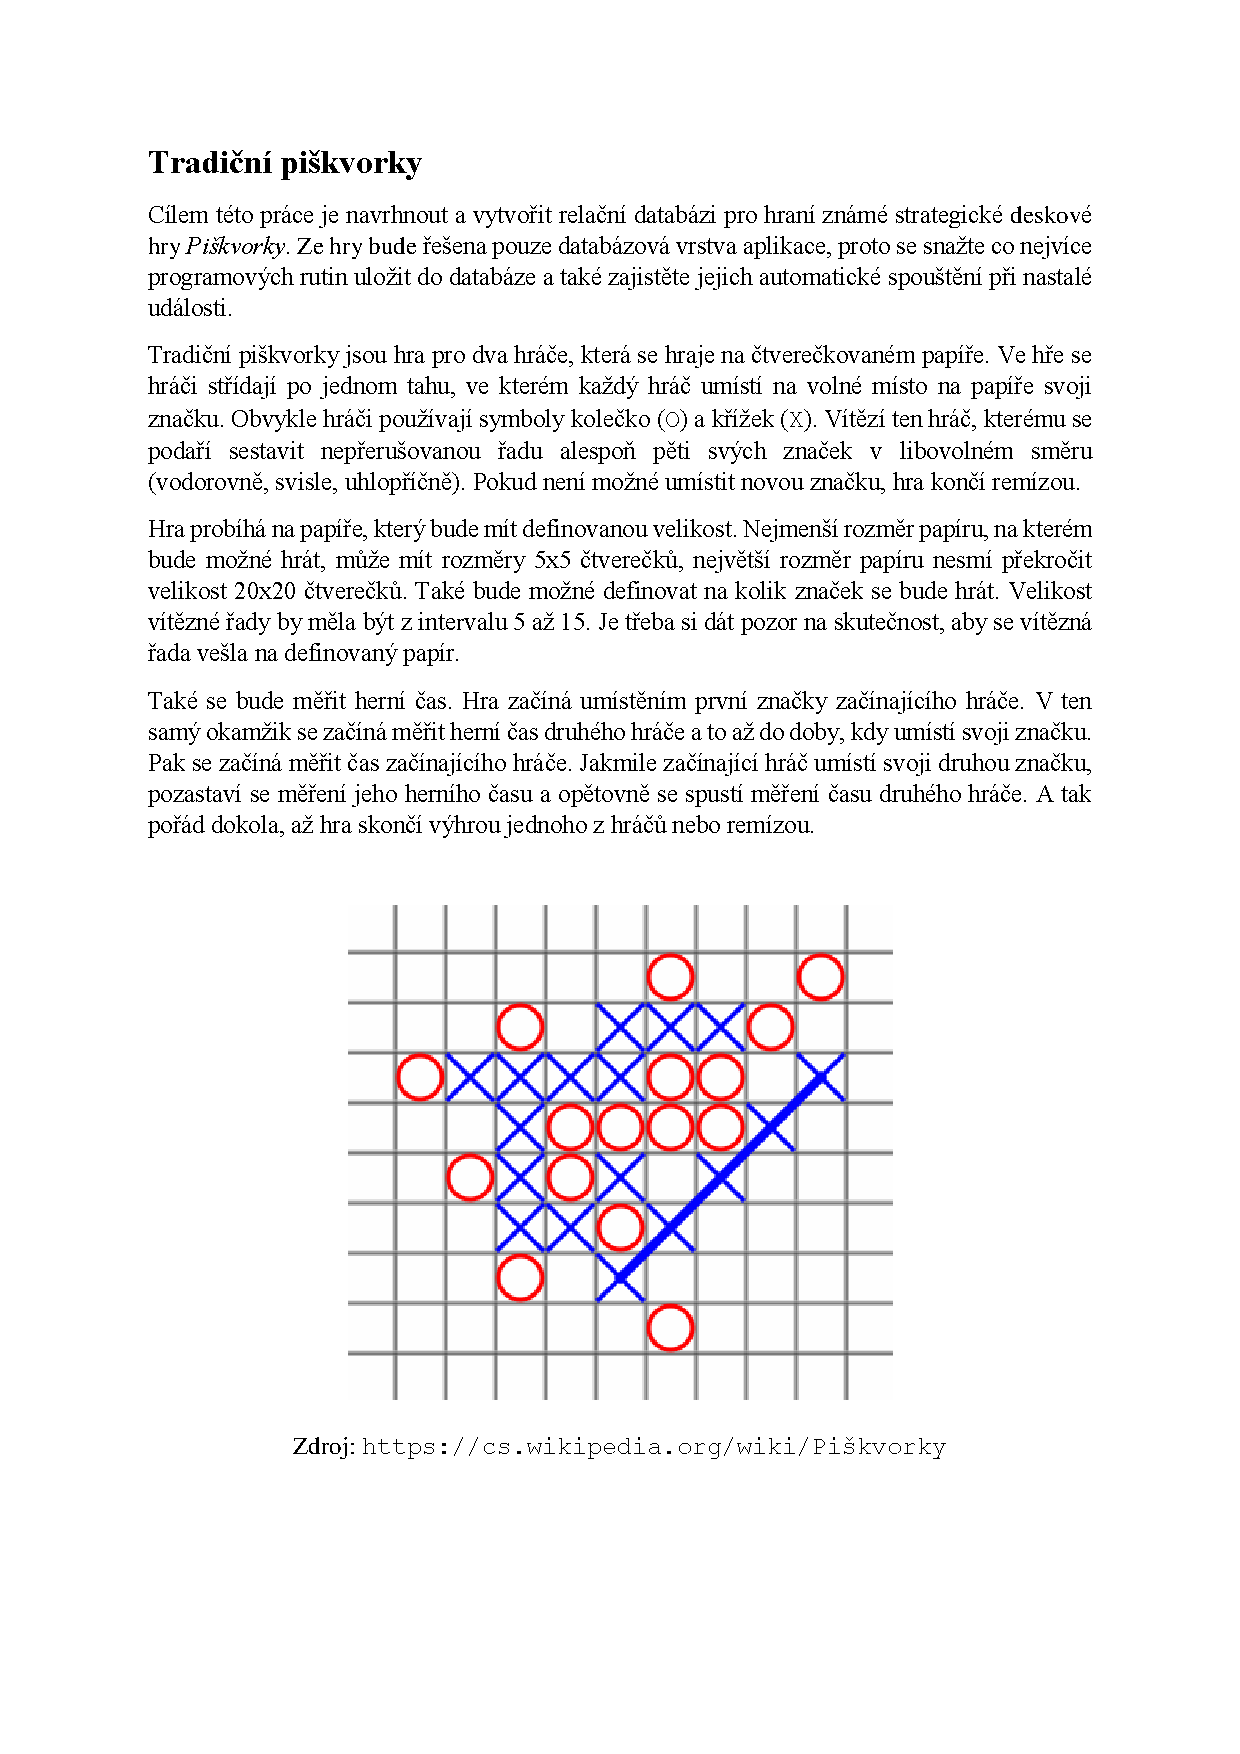
\includepdf[pages=1,pagecommand=\section{Zadání}, offset=0 -3cm]{specification.pdf}
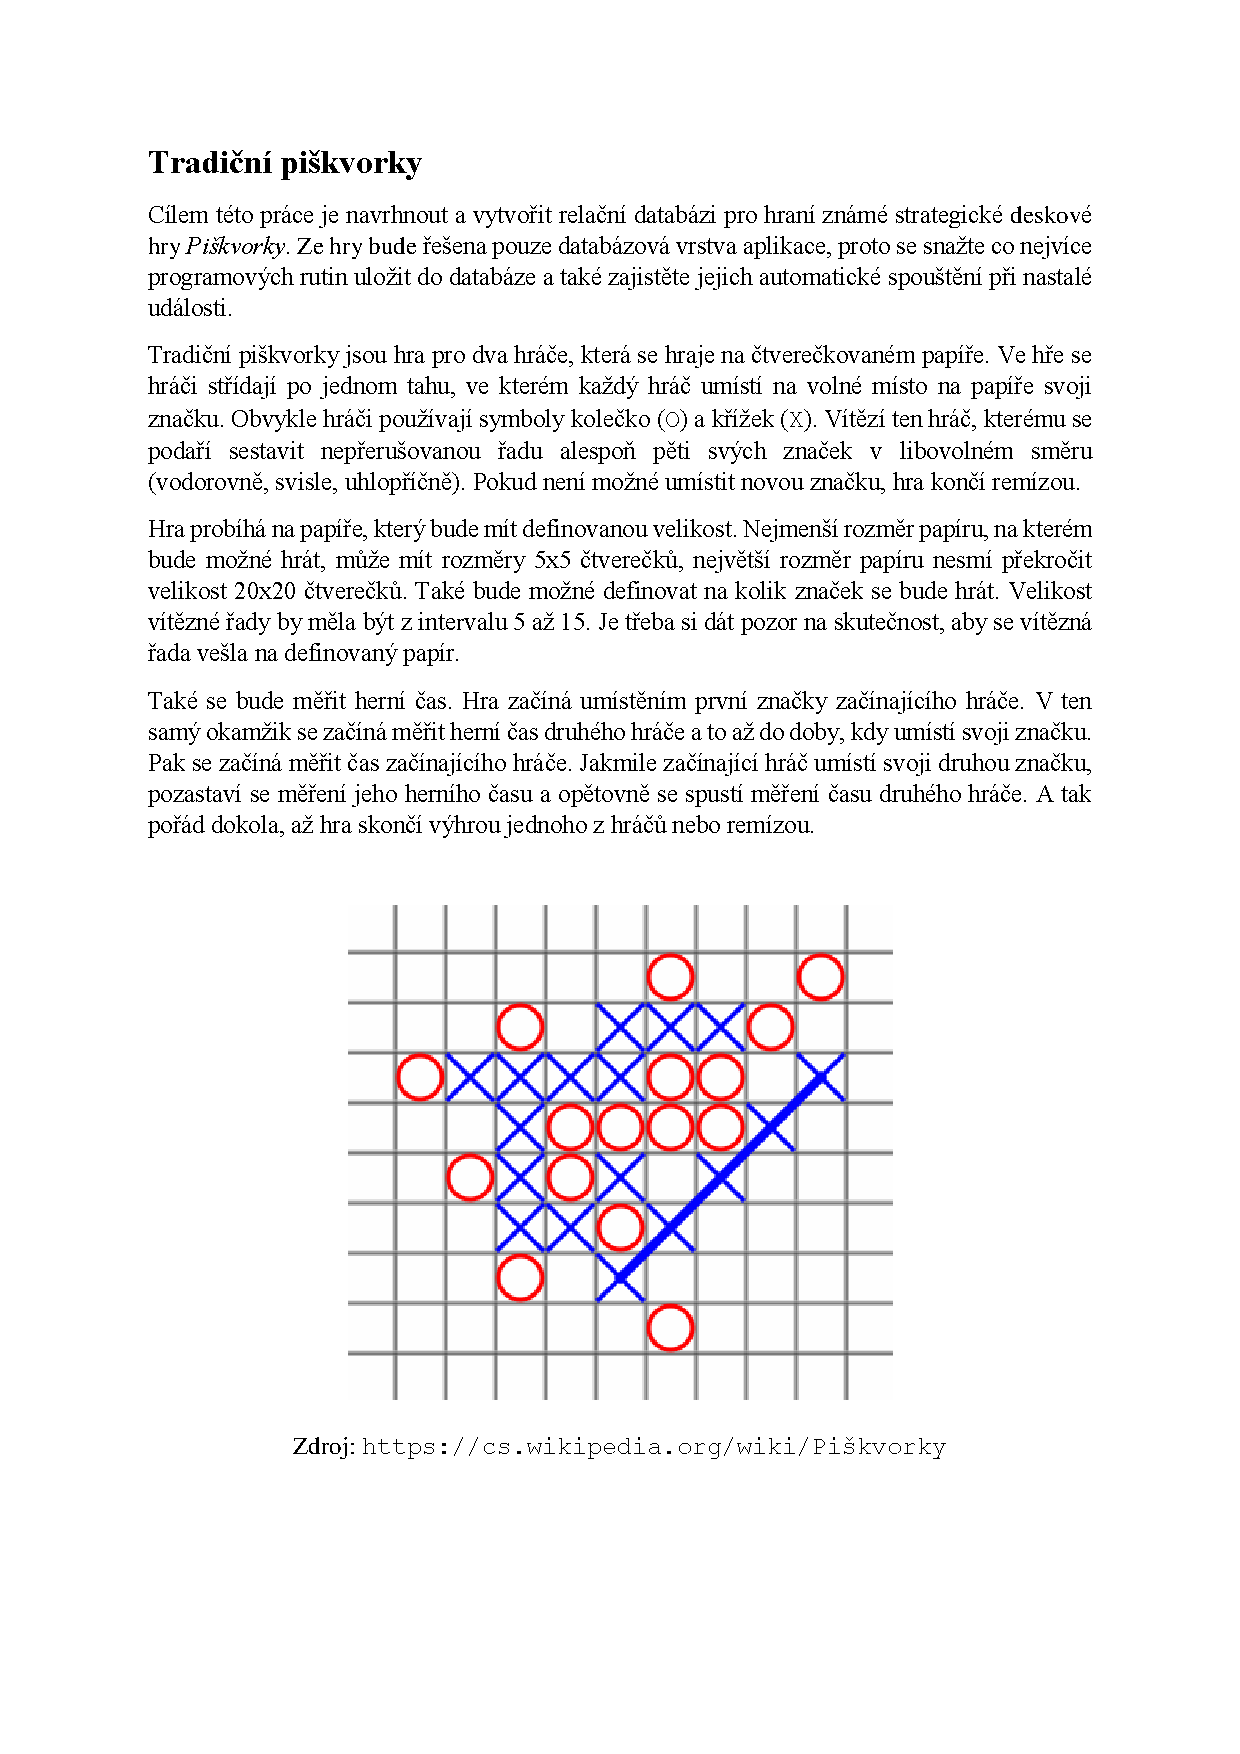
\includepdf[page={2,3,4}]{specification.pdf}

\section{Datová analýza}
Datový model semestrální práce obsahuje celkem 6 tabulek. Všechny tabulky mají definovaný primární klíč s názvem ID. Integrita databáze je zajištěna.
Diagram datového modelu je zobrazen na obrázku \ref{fig:model}.
\begin{figure}[h]
	\centering
	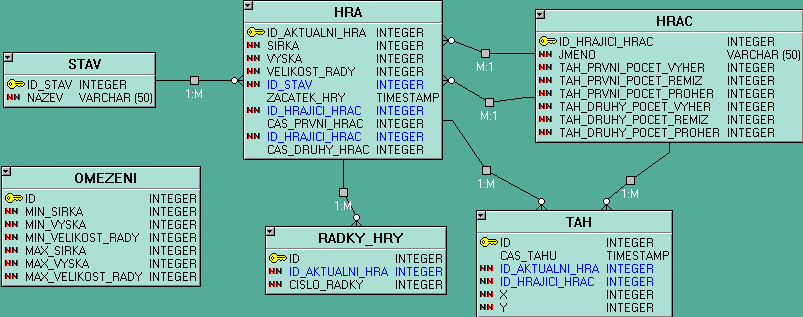
\includegraphics[width=1\linewidth]{img/data_model.png}
	\caption{ER diagram datového modelu.}
	\label{fig:model}
\end{figure}

\section{Funkční analýza}
	\subsection{Vybrané pohledy}
		\subsubsection{Pohled PAPIR}
		Pohled \textbf{PAPIR} zobrazí všechny řádky na papíru i se všemi značkami v dané hře. Začínající hráč má vždy přiřazenou značku "\textbf{O}" a druhý hráč má přiřazenou značku "\textbf{X}". Řádky jsou od sebe odděleny značkou "\textbf{|}". Funkční SQL kód viz kód \ref{lst:view_papir}.

		\begin{lstlisting}[caption = {SQL kód pohledu \textbf{PAPIR}.}, label = {lst:view_papir}, captionpos=b, frame=single]
CREATE OR REPLACE VIEW PAPIR(ID_HRA) AS
SELECT 
	ID_HRA, 
	CISLO_RADKY,
	RADEK_PAPIRU(ID_HRA, CISLO_RADKY)
FROM RADKY_HRY;
		\end{lstlisting}

		\subsubsection{Pohled REMIZY}
		Pohled \textbf{REMIZY} zobrazí všechny ukončené hry, které skončili remízou. Každý řádek obsahuje:
		\begin{itemize}
		\item ID hry
		\item šířka papíru
		\item výška papíru
		\item velikost vítězné řady
		\item celková doba hraní hry
		\item jméno prvního hráče
		\item jméno druhého hráče
		\end{itemize}
		Při zobrazování se používá tabulka \textit{HRA}, ke které se napojí tabulka \textit{HRAC}. Funkční SQL kód viz kód \ref{lst:view_remizy}.

		\begin{lstlisting}[caption = {SQL kód pohledu \textbf{REMIZY}.}, label = {lst:view_remizy}, captionpos=b, frame=single]
CREATE OR REPLACE VIEW REMIZY AS
SELECT 
	HRA.ID AS ID_HRY, 
	HRA.SIRKA, 
	HRA.VYSKA, 
	HRA.VELIKOST_RADY, 
	CAS_PRVNI_HRAC + CAS_DRUHY_HRAC 
	AS DOBA_HRANI_HRY,
	H1.JMENO AS ZACINAJICI_HRAC,
	H2.JMENO AS DRUHY_HRAC
	FROM HRA
		LEFT JOIN HRAC AS H1
		ON H1.ID = HRA.ID_PRVNI_HRAC
		LEFT JOIN HRAC AS H2
		ON H2.ID = HRA.ID_DRUHY_HRAC	
	WHERE REMIZA(HRA.ID);
		\end{lstlisting}

	\subsection{Vybraná funkce}
		\subsubsection{Funkce REMIZA}
		\label{function_remiza}

		Funkce \textbf{REMIZA} kontroluje stav hry. Pokud je stav hry roven 4, je vráceno \textit{TRUE}. V ostatních případech je vrácená hodnota \textit{FALSE}. Funkční SQL kód viz kód \ref{lst:function_remiza}.
		\begin{lstlisting}[caption = {SQL kód funkce \textbf{REMIZA}.}, label = {lst:function_remiza}, captionpos=b, frame=single]
CREATE OR REPLACE FUNCTION REMIZA(ID_HRA INTEGER) 
RETURNS BOOLEAN AS $$
	DECLARE
		I_HRA HRA;
	BEGIN
		SELECT * INTO I_HRA FROM HRA 
		WHERE ID = ID_HRA;
		IF I_HRA.ID_STAV = 4 THEN
			RETURN TRUE;
		END IF;
		
		RETURN FALSE;
	END;
	$$ LANGUAGE plpgsql;
		\end{lstlisting}

	\subsection{Vybraná procedura}
		\subsubsection{Procedura KONEC\_HRY}
		\label{procedure_konec_hry}

		Procedura \textbf{KONEC\_HRY} kontroluje stav hry. Procedura v případě, že stav hry je roven 1, tak vypočítá herní dobu obou hráčů a následně tyto hodnoty vloží do tabulky \textbf{HRA}. Funkční SQL kód viz kód \ref{lst:procedure_konec_hry}.
\newpage
		\begin{lstlisting}[caption = {SQL kód procedury \textbf{KONEC\_HRY}.}, label = {lst:procedure_konec_hry}, captionpos=b, frame=single]
CREATE OR REPLACE PROCEDURE KONEC_HRY (ID_HRA INTEGER) 
AS $$
	DECLARE
		I_HRA HRA;
	BEGIN
		SELECT * INTO I_HRA FROM HRA WHERE 
		ID = ID_HRA;
		
		IF I_HRA.ID_STAV = 1 THEN
			RETURN;
		END IF;
		UPDATE HRA SET CAS_PRVNI_HRAC = 
		HERNI_CAS(I_HRA.ID, I_HRA.ID_PRVNI_HRAC)
		, CAS_DRUHY_HRAC = 
		HERNI_CAS(I_HRA.ID, I_HRA.ID_DRUHY_HRAC) 
		WHERE ID = ID_HRA;
	END;
	$$ LANGUAGE plpgsql;	
		\end{lstlisting}

	\subsection{Vybraný trigger}
		\subsubsection{Trigger HRA\_DOHRANA}
		Trigger \textbf{HRA\_DOHRANA} se spustí vždy po úpravě stavu hry. Trigger poté volá funkce \textbf{VYHRA} a \ref{function_remiza}. Pokud alespoň jedna z těchto funkcí vrátí hodnotu \textit{TRUE}, tak se provede ukončení hry voláním procedur \ref{procedure_konec_hry} a \textbf{STATISTIKY}. Funkční SQL kód viz kód \ref{lst:trigger_hra_dohrana}.
\newpage
		\begin{lstlisting}[caption = {SQL kód triggeru \textbf{HRA\_DOHRANA}.}, label = {lst:trigger_hra_dohrana}, captionpos=b, frame=single]
CREATE OR REPLACE FUNCTION VYTVOR_TRIGGER_HRA_DOHRANA() 
RETURNS TRIGGER AS $VYTVOR_TRIGGER_HRA_DOHRANA$
	DECLARE
	BEGIN		
		IF VYHRA(NEW.ID) = TRUE 
		OR REMIZA(NEW.ID) = TRUE THEN
			CALL KONEC_HRY(NEW.ID);
			CALL STATISTIKY(NEW.ID);
		END IF;

		RETURN NEW;
	END;
	$VYTVOR_TRIGGER_HRA_DOHRANA$ LANGUAGE plpgsql;	
	
CREATE TRIGGER HRA_DOHRANA AFTER UPDATE OF ID_STAV 
ON HRA FOR EACH ROW EXECUTE PROCEDURE 
VYTVOR_TRIGGER_HRA_DOHRANA();
		\end{lstlisting}

\section{Testovací scénář}
Pro zahájení hry je potřeba vložit záznam do tabulky \textbf{HRA}. Příklad vytvoření nové hry viz Listing \ref{lst:insert_hra}.
		\begin{lstlisting}[caption = {Příklad vložení záznamu do tabulky \textbf{HRA}.}, label = {lst:insert_hra}, captionpos=b, frame=single]
INSERT INTO HRA(SIRKA, VYSKA, VELIKOST_RADY, 
ID_PRVNI_HRAC, ID_DRUHY_HRAC) VALUES (20, 20, 5, 1, 2);
		\end{lstlisting}

Jakmile se hra vytvoří, tak může začínající hráč provést svůj první tah (pokud se bude snažit vložit tah druhý hráč ještě předtím, než vloží tah začínající hráč, tak mu to trigger \textbf{ZKONTROLUJ\_TAH} zakáže a vyhodí vyjímku). Příklad provedení tahu viz Listing. \ref{lst:insert_tah}.
		\begin{lstlisting}[caption = {Příklad vložení záznamu do tabulky \textbf{TAH}.}, label = {lst:insert_tah}, captionpos=b, frame=single]
INSERT INTO TAH(ID_AKTUALNI_HRA, ID_HRAJICI_HRAC, X, Y) 
VALUES (2, 1, 1, 1);
		\end{lstlisting}

Pro zobrazení celého papíru se zavolá pohled \textbf{PAPIR} pomocí příkazu \textit{SELECT} se zadaným ID hry, pro kterou chceme zobrazit papír.
Pro zobrazení her, ve kterých vyhrál nebo prohrál začínající hráč, se zavolají pohledy \textbf{VYHRY\_ZACINAJICI, PROHRY\_ZACINAJICI} pomocí příkazu \textit{SELECT}.
Pro zobrazení her, které skončili remízou, se zavolá pohled \textbf{REMIZY} pomocí příkazu \textit{SELECT}.


\section{Závěr}
Semestrální práce splňuje zadanou funkcionalitu. Po vložení nového záznamu do tabulky \textbf{TAH} jsou triggery schopny rozpoznat, zda daný hráč vytvořil řadu po sobě jdoucích značek o dané velikosti a následně na to zareagovat ukončením hry a aktualizováním statistik. Pro potřeby výpisu daného řádku hry bylo potřeba vytvořit navíc tabulku \textbf{RADKY\_HRY}, kde každý záznam reprezentuje pár ID hry - Číslo řádky. V semestrální práci byly implementovány všechny požadované funkce, procedury, pohledy a tabulky, které jsou používány triggery. Navíc bylo vytvořeno 5 testovacích scénářů, pomocí kterých byla otestována funkčnost kontroly stavu hry.
	
\end{document}